\chapter{System Requirements Analysis and Design}
\section{The System Context Analysis}

\begin{figure}[H]
    \centering
    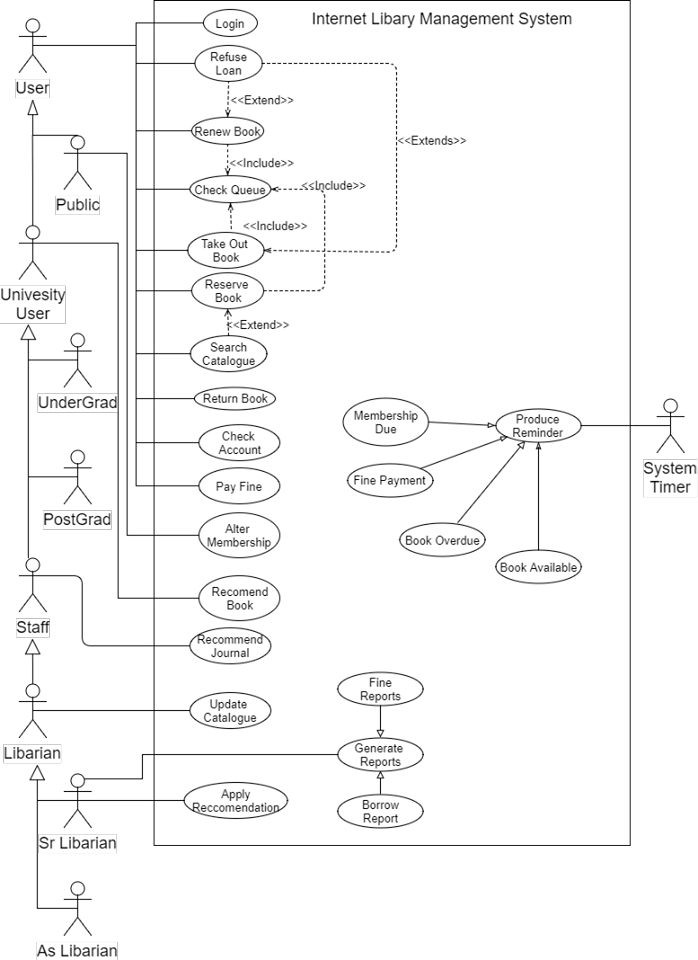
\includegraphics[width=0.8\linewidth]{image/use_cases.png}
    \caption{Use Case Diagram}
    \label{fig:usecase}
\end{figure}

\subsection{Purpose for Use Case Model}

The Use Case Model describes the proposed functionality of a new system and serves as a contract between the end user and the developers. It represents a list of actions or event steps typically defining the interactions between a role (known as an actor) and a system to achieve a goal. An actor is a human or machine entity that interacts with the system. The model consists of Constraints, Requirements and Scenarios. Each Use Case has a description which describes the functionality that will be built in the proposed system and it may `include' another Use Case's functionality or `extend' another Use Case with its own behaviour\cite{umlusecase}. Use cases serve as a unifying thread throughout system development. The same use-case model is the result of the Requirements discipline, and is used as input to Analysis \& Design and Test disciplines. Use case diagrams are a benefit to modelling of the system as they can show who interacts with the system and what they can interact with. Different tiers of actors (For example a user and an admin) will have different access limitations and therefore have different use cases (although most will be shared). Both a user and an admin will be able to take a book out as shown on the diagram but only a member of staff will be able to recommend a journal. The use case model summarises every action possible of each actor and will give an overview of which actor can access different actions. This is an important aspect when developing the system\cite{eclipseusecase}.

The use case model will play a key part in designing and building the system, it will give an outline of all actions the system can handle and therefore the system will be easier to plan. It will also be used to prioritise work being able to view more important use cases and actors. It can also ensure that the system delivered works properly\cite{alhirusecase}.

\subsection{Summary of Actors}

There are a large number of distinct actors that need to interact with the system. Each of these has been distinguished as a result of necessary specialisation. The first core decision made was to have all actors inherit one core actor type ``User''. This decision was made as all accounts will share some common functionality, be they Librarians who act as Administrators, or Public users who are the least privileged in the system. This has the side effect of including Librarians in the main hierarchy, meaning that they will have one unified account which they can use to take out books and interface with the library as a normal user, rather than having a separate account as a user and as an administrator. This is both positive and negative. On the one hand it means that as they are not switching accounts for different functions, librarians will have an easier time using the system, but it also removes an element of separation of concerns.

\subsection{Conditions}

\begingroup
\def\arraystretch{1.5}
\begin{longtabu}{>{\bfseries}r X}
    C1 & is the condition that will check that the membership length does not contradict the loan length. An example of this is when a user would try to borrow a book for 30 days, but they only have 18 days left on their membership. This condition would be flagged and the loan would be refused and the process stopped. \\
    C2 & is the condition that you have an outstanding fine to pay. An example of when this would be flagged as true would be when a user attempts to renew a book but they have had the book over their loan length limit. They will be flagged as having a fine to pay and will be not allowed to renew the book. \\
    C3 & is the condition that checks the loan limits. This condition would be flagged if the user attempts to take out another book while they are already at their maximum limit books. \\
    C4 & is the condition that the book currently has a hold by another user in the reservation queue. An example of this being flagged is when a user attempts to renew a book that has been put on hold for another user. \\
    C5 & is the condition that the user has a book or multiple books overdue for return to the library.  \\
    C6 & is the condition that the user has entered valid login credentials this includes a correct username and the correct corresponding password for an account. \\
    C7 & a user can only reserve a book up to five times. \\
    C8 & is the condition whether a user has reached their maximum renew limit. An example of this being flagged is when a user tries to renew a book but has reached their limits they will not be allowed to renew the book. \\
    C9 & If the user membership is less than 30 days then stop recommendation privileges. \\
    C10 & if a user wishes to cancel their membership they must not have any outstanding items nor outstanding fines. \\
    C11 & User has a reserved book available to collect. \\
\end{longtabu}
\endgroup

\subsection{Actors}

\begingroup
\def\arraystretch{1.5}
\begin{longtabu}{>{\bfseries}r X}
    User & is an abstract actor, representing the functionality available to all members of the system. This includes Login, Renew Book, Check Queue, Take Out Book, Reserve Book, Search Catalogue, Return Book, Check Account, and Pay Fine. \\
    Public & represents a member of the public who has joined the library from outside the university. They have access an additional Alter Membership use case. \\
    University User & is an abstract actor, representing the functionality available to all non public members of the system i.e. the Recommend Book use case. \\
    Undergrad & represents an undergraduate student, they are distinct in the system due to the specialisation on the number of books they can withdraw. \\
    Postgrad & represents a postgraduate student, they are distinct in the system due to the specialisation on the number of books they can withdraw. \\
    Staff & represents a member of staff at the university, they are able to Recommend Journals and Magazines in addition to just Books. They also have specialisation on number of books they can withdraw. \\
    Librarian & is an abstract actor, representing all librarians. They have access to the Update Catalogue Functionality. \\
    Sr Librarian & represents a Senior Librarian, they have the ability to approve book, journal, and magazine recommendations set out by other users. \\
    As Librarian & represents an Assistant Librarian, they are a concrete implementation of Librarian without the added functionality of a Senior Librarian.
\end{longtabu}
\endgroup

\pagebreak
\subsection{Use Case Descriptions}

\begingroup
\def\arraystretch{1.5}
\begin{longtabu}{>{\bfseries}r X}
    Login & allows the user to provide a username and password as a gateway in order to interface with the system. \\ & Conditions: C6 \\
    Renew Book & allows a user to renew a book that they have taken out. \\ & Conditions: C1, C2, C4, C8 \\
    Check Queue & checks if the book currently has a queue of users who have reserved a specific book.  \\ & Conditions: C4 \\
    Take Out Book & allows the user to take out a book from the library. \\ & Conditions: C1, C2, C3, C4, C5 \\
    Reserve Book & gives the user the option to out a book on hold for them. \\ & Conditions: C4, C7 \\
    Search Catalogue & allows the user to search the catalogue of the books that the library has. \\ & Conditions:C9 \\
    Refuse Loan & refuses a loan of a book when certain conditions are not met by the user. \\
    Return Book & allows a user with a borrowed book to return that book. \\ & Conditions: C5, C9 \\
    Check Account & allows the user to check details related to their account. \\ & Conditions: C6 \\
    Pay Fine & allows the user to pay any fine expected of them. \\ & Conditions: C2, C5 \\
    Alter Membership & allows a public member to alter their membership. \\ & Conditions:C6 \\
    Recommend Book & allows a user to recommend a book for purchase. \\ & Conditions: C9 \\
    Recommend Journal & allows specific users to recommend journals for purchase. \\ & Conditions: C9 \\
    Update Catalogue & allows the user to manipulate the library’s book database. \\
    Apply Recommendation & allows specific users to apply the intended book recommendation for purchase. \\ & Conditions: C9 \\
    \pagebreak Generate Report & will generate specific types of management reports. \\ & Conditions: No conditions, no triggers. (Requests via Librarian) \\
    Fine Report & produces a report of the fine and the breakdown of the fine. \\ & Conditions: No conditions, no triggers. (Requests via Librarian) \\
    Borrow Report & produces a report of the books that are borrowed and when the book needs to be returned. \\ & Conditions: No conditions, no triggers. (Requests via Librarian) \\
    Produce Reminder & will send produce reminders directly sent to the user. \\ & Conditions: No conditions, triggered via membership due, fine payment, book overdue, book available.  \\
    Membership Due & public users will receive information regarding when their membership is due.  \\ & Conditions: C9 \\
    Fine Payment & produces a reminder that a user has a fine that needs to be dealt with. \\ & Conditions: C2 \\
    Book Overdue & produces a reminder that a user has a book overdue. \\ & Conditions: C5 \\
    Book Available & sends a reminder to a user that a specific book is now available. \\ & Conditions: C11
\end{longtabu}
\endgroup

\subsection{Use Case Description}
\begingroup
\def\arraystretch{1.5}
\begin{longtabu}{|r|X|}
    \hline
    Use Case Name & Take Out Book \\\hline
    ID & 1 \\\hline
    Importance & 1 / Core Function \\\hline
    Description & Allows a user to take out a book from the library. \\
    & If successful: updates the user’s recorde as well as the record for the copy of the book, with details of the loan. Also changes associated attributes of both the user record and book copy (i.e: number of loans available; on shelf to out on loan). \\
    & If Unsuccessful: prints message to screen stating loan has been denied and why. Returns user to previous menu. \\\hline
    Actors & User \\\hline
    Triggers & Actor Input --- passes book, user profile. \\\hline
    Conditions & Use account can borrow: \begin{itemize}
        \item Has $>0$ additional loans available
        \item Is not blocked from borrowing (fines outstanding)
        \item Has valid membership
    \end{itemize} \\
    & Remaining membership $>$ book loan period\\
    & Copy of book can be borrowed:\begin{itemize}
        \item Is on shelf (i.e. not out / on hold)
    \end{itemize} \\\hline
    Relationship & Is extended by refuse loan. \\
    & Associated with actor type User. \\\hline
    Flow of Events & Request TakeOutBook() \\
    & Check if membership is valid for more than 30 days \\
    & If membership is not valid, inform user ``invalid membership'' and stop process \\
    & Else check fines, \\
    & If outstanding fines, inform user ``outstanding fines'' and stop process \\
    & Else check loan limits \\
    & If user is at their loan limit, inform user reached ``loan limit reached'' and stop process \\
    & Else continue update actions in parallel \\
    & Calculate timestamp of action and return date for the book \\
    & Update loan status on user account \\
    & Alter status of book to “on loan” \\
    & Remove one copy of book from ILMS system \\
    & Add one book to the user’s loan limit \\
    & Confirm the request to take out book \\
    & Stop \\\hline
    Alternatives / Exceptions & Ammend loan length: \\
    & dueDate = user.membershipEndDate; \\
    & Refuse loan: \\
    & Print to screen appropriate message; \\
    & Return; \\\hline
\end{longtabu}
\endgroup

The output of use case analysis is vital for the creation of activity diagrams, as well as effectively modelling the features of a single function that the ILMS will complete. Use case models are utilised as the primary specification for the functional requirements of the system, combined with the basis for analysis and design as an input to iteration planning, defining test cases and for user documentation\cite{usecaseanalliu}.